\documentclass[a4paper,11pt]{article}
\usepackage{amsmath,amsthm,amsfonts,amssymb,amscd,amstext,vmargin,graphics,graphicx,tabularx,multicol} 
\usepackage[francais]{babel}
\usepackage[utf8]{inputenc}  
\usepackage[T1]{fontenc} 
\usepackage{pstricks-add,tikz,tkz-tab,variations}
\usepackage[autolanguage,np]{numprint} 
\usepackage{calc}

\setmarginsrb{1.5cm}{0.5cm}{1cm}{0.5cm}{0cm}{0cm}{0cm}{0cm} %Gauche, haut, droite, haut
\newcounter{numexo}
\newcommand{\exo}[1]{\stepcounter{numexo}\noindent{\bf Exercice~\thenumexo} : }
\reversemarginpar

\newcommand{\bmul}[1]{\begin{multicols}{#1}}
\newcommand{\emul}{\end{multicols}}

\newcounter{enumtabi}
\newcounter{enumtaba}
\newcommand{\q}{\stepcounter{enumtabi} \theenumtabi.  }
\newcommand{\qa}{\stepcounter{enumtaba} (\alph{enumtaba}) }
\newcommand{\initq}{\setcounter{enumtabi}{0}}
\newcommand{\initqa}{\setcounter{enumtaba}{0}}

\newcommand{\be}{\begin{enumerate}}
\newcommand{\ee}{\end{enumerate}}
\newcommand{\bi}{\begin{itemize}}
\newcommand{\ei}{\end{itemize}}
\newcommand{\bp}{\begin{pspicture*}}
\newcommand{\ep}{\end{pspicture*}}
\newcommand{\bt}{\begin{tabular}}
\newcommand{\et}{\end{tabular}}
\renewcommand{\tabularxcolumn}[1]{>{\centering}m{#1}} %(colonne m{} centrée, au lieu de p par défault) 
\newcommand{\tnl}{\tabularnewline}

\newcommand{\trait}{\noindent \rule{\linewidth}{0.2mm}}
\newcommand{\hs}[1]{\hspace{#1}}
\newcommand{\vs}[1]{\vspace{#1}}

\newcommand{\N}{\mathbb{N}}
\newcommand{\Z}{\mathbb{Z}}
\newcommand{\R}{\mathbb{R}}
\newcommand{\C}{\mathbb{C}}
\newcommand{\Dcal}{\mathcal{D}}
\newcommand{\Ccal}{\mathcal{C}}
\newcommand{\mc}{\mathcal}

\newcommand{\vect}[1]{\overrightarrow{#1}}
\newcommand{\ds}{\displaystyle}
\newcommand{\eq}{\quad \Leftrightarrow \quad}
\newcommand{\vecti}{\vec{\imath}}
\newcommand{\vectj}{\vec{\jmath}}
\newcommand{\Oij}{(O;\vec{\imath}, \vec{\jmath})}
\newcommand{\OIJ}{(O;I,J)}


\newcommand{\reponse}[1][1]{%
\multido{}{#1}{\makebox[\linewidth]{\rule[0pt]{0pt}{20pt}\dotfill}
}}

\newcommand{\titre}[5] 
% #1: titre #2: haut gauche #3: bas gauche #4: haut droite #5: bas droite
{
\noindent #2 \hfill #4 \\
#3 \hfill #5

\vspace{-1.6cm}

\begin{center}\rule{6cm}{0.5mm}\end{center}
\vspace{0.2cm}
\begin{center}{\large{\textbf{#1}}}\end{center}
\begin{center}\rule{6cm}{0.5mm}\end{center}
}



\begin{document}
\pagestyle{empty}
\titre{Séance d'AP 2 : Différentes numérations}{}{}{6ème}{}

\vspace*{0.5cm}

\textbf{{\large A. Numération romaine (27 avant J-C / 476 après J-C)} }\\

Ce système, qui simplifiait les anciennes numérations grecques et phéniciennes, permet d'écrire tous les nombres de 1 à 4999, en utilisant les lettres de l'alphabet latin.\\
Néanmoins ce système ne les a pas remplacés totalement, car il était trop simplifié et insuffisant pour exprimer tous les
nombres.\\

Voici le tableau de correspondance:
\renewcommand{\arraystretch}{1.3}

\begin{center}
\begin{tabular}{|c|m{1cm}|m{1cm}|m{1cm}|m{1cm}|m{1cm}|m{1cm}|m{1cm}|}
\hline 
Chiffre romain & I \hspace*{0.2cm}& V & X & L & C & D & M \\ 
\hline 
Valeur &  &  &  &  &  &  &  \\ 
\hline 
\end{tabular} 

\end{center}

\vspace*{0.3cm}

La complexité du système romain apparaît déjà dans les exemples suivants :\\

\includegraphics[scale=0.50]{tabchiffreromain.eps} 

\vspace*{0.3cm}

Pour connaître la valeur d'un nombre écrit en chiffres romains, il faut lire le nombre de droite à gauche, il suffit d'ajouter la valeur du chiffre, sauf s'il est inférieur au précédent, dans ce cas, on le soustrait. \\

Quelques exemples pour comprendre :\\

\bi
\item XVI = 1 + 5 + 10 = 16\\

\item XIV = 5 - 1 + 10 = 14\\

\item MMMMCMXCIX = 10 - 1 + 100 - 10 + 1 000 - 100 + 1 000 $\times$ 4 = 4 999\\

\ei


\vspace*{0.5cm}

\textbf{\underline{A toi de jouer !}}\\



\initq \q Quels sont les nombres suivants ?\\

XIII = \hspace*{3cm}  DIX = \hspace*{3cm} MCMLXXXIV = \\

MDCXXXVIII (Année de naissance de Louis XIV) = \\



\newpage


\q Écrire les nombres suivants en numération romaine :

\bmul{2}

476 (Chute de l'empire romain) = \\


\columnbreak


1754 (Année de naissance de Louis XVI) =\\

\emul

. . . . . . (Votre année de naissance) =\\

\q Quel est le nombre en chiffres romains le plus long en quantité de symboles ? . . . . . . . . . . . . .\\ 



\textbf{{\large B. La numération maya (environ 300 ans après J-C) }}\\


En Amérique centrale, les Mayas utilisaient un système dit de " base 20" qui ne comprenait que trois signes.\\

Pour eux, le zéro était représenté par 
\includegraphics[scale=0.5]{maya1.eps} , l'unité par 
\includegraphics[scale=0.55]{maya3.eps} et le nombre 5 par 
\includegraphics[scale=0.55]{maya2.eps} .\\
Ces symboles permettent d'écrire tous les nombres de 0 à 19, comme le montre le tableau ci-dessous.

\begin{center}
\includegraphics[scale=0.75]{maya4.eps} 
\end{center}


Pour les nombres plus grands que 19, les Mayas écrivaient les nombres sur plusieurs étages (de bas en haut), utilisant les puissances de 20. Des exemples :\\

\textit{Lire un nombre maya :}				\hspace*{7cm}			\textit{Écrire un nombre en maya :}\\
 \includegraphics[scale=0.6]{maya7.eps} \hspace*{2cm}	  \includegraphics[scale=0.8]{maya11.eps} \\
 

\textbf{\underline{A toi de jouer !}}\\


\initq \q Compléter le tableau de numération ci-dessus.\\

\q Quels sont les nombres suivants (Faire apparaître vos calculs dans votre réponse):\\


\includegraphics[scale=0.6]{maya8.eps}  \hspace*{4.5cm}
\includegraphics[scale=0.6]{maya9.eps}  \hspace*{4.5cm} 
\includegraphics[scale=0.6]{maya10.eps} \\


\q Ecrire les nombres suivants en numération Maya :\\

36 = \hspace*{8cm}  68 = \\

\vspace*{1cm}

432 = \hspace*{8cm}  2018 = \\





\end{document}
